\documentclass[12pt]{article}
\usepackage{sbc-template}
\usepackage{graphicx,url}
\usepackage[utf8]{inputenc}
\usepackage[brazilian]{babel}
\usepackage{float}
\usepackage{array}
\usepackage{amsmath,amssymb}

\sloppy

\title{Predição de criminalidade contra pessoas trans e travestis: \\ Relação entre notificações de violência e indicadores municipais no Brasil}

\author{Ana Queiroz da Silva, Natália Metolina, Pedro Henrique Teixeira Soares}

\address{Escola de Artes, Ciências e Humanidades -- Universidade de São Paulo (USP)\\
Rua Arlindo Bétio nº 1000 -- São Paulo -- SP -- Brasil}

  
\begin{document}

\maketitle
     
\begin{resumo}
A violência contra pessoas trans e travestis no Brasil tem pouca visibilidade nas bases oficiais, que raramente separam essa população do conjunto LGBT. Este trabalho usa as denúncias do Disque 100 de 2011 a 2022 (27.441 registros de vítimas LGBT em 2.070 municípios), combinadas a indicadores do IBGE, da pesquisa MUNIC, do Atlas da Violência e do SUS, para identificar os municípios com números alarmantes e prever onde tendem a surgir ondas de denúncias. Depois de unificar os três formatos de registro da base e descontar o porte de cada cidade, 141 municípios tiveram números alarmantes em 2020--2022, 83 deles com menos de 100 mil habitantes. Na previsão de um ano à frente, o LightGBM reduziu o erro em 16,7\% (IC 95\%: 13,3--20,3) em relação a distribuir as denúncias apenas pela população e, monitorando 1\% dos municípios, concentrou 31\% das ondas, contra 22\% da referência. As denúncias foram mais frequentes onde há mais casais do mesmo sexo, maior densidade demográfica e ouvidoria municipal de direitos humanos, e as ondas permaneceram locais, sem se espalhar para cidades vizinhas. As vítimas trans foram 18\% das denúncias com identidade registrada e sofreram violência mais grave e mais pública: em violações contra a vida, a chance de a vítima ser trans foi três vezes maior. Não foi possível medir efeito da criminalização da transfobia pelo STF em 2019: a queda nas denúncias trans começou meses antes e acompanha mudanças no registro, que pesaram mais nos números do que o marco legal.

\textbf{palavras-chave:} violência contra população trans; pessoas trans e travestis no Brasil; Disque 100; previsão espaço-temporal; aprendizado de máquina.
\end{resumo}


\section{Introdução}

A produção de dados referentes à população trans no Brasil é um desafio persistente e uma limitação para a elaboração de políticas públicas. Os Censos elaborados pelo Intituto de Geografia e Estatística (IBGE) não apresentam dados especializados referentes à identidade de gênero. A população transgênera é definida como o conjunto de pessoas que se identificam com um gênero incongruente ou diferente daquele que lhes foi atribuído ao nascer e estima-se que representam entre 0.1\% a 2\% da população brasileira, a depender da localidade. Estima-se que o total da população transgênera no Brasil se distribua da seguinte forma: Norte 8\%, Nordeste 26\%, Centro-Oeste 7\%, Sudeste 44\% e Sul 15\ \cite{spizziri_eufrasio_lima:2021}. Travestis  são uma identidade de gênero revindicada na América Latina, reunindo pessoas designadas como do sexo masculino ao nascer, mas que se identificam com o feminino, embora não necessariamente se identifiquem como mulheres \cite{leal_silva_lizzi:2026}. Para fins de pesquisa abarcaremos as categorias "transgênero", "travesti" e "transexual", esta última presente em bases de dados e documentos oficiais dos programas de saúde públicos, atendendo as diversas fontes utilizadas no trabalho.

A violência é um fenômeno complexo e polissêmico, sendo delimitado neste trabalho às definições presentes na Classificação Internacional de Doenças, caracterizando-se pelo uso intencional da força ou poder que possa ocasionar lesão, morte, privação, deficiência ou dano psicológico \cite{marinho_tomazelli_firianelli:2024}. Em 2011 a notificação de violência autoprovocada e interpessoal integrou a lista de notificação compulsória e foi incluída no Sistema de Informação de Agravos de Notificação (Sinan) e em 2014, para contemplar a Política Nacional de Saúde Integral de Lésbicas, Gays, Bissexuais, Travestis e Transexuais, foram incluídas na ficha de notificação as variáveis “orientação sexual”, “identidade de gênero” e "nome social". Em 2019, o Supremo Tribunal Federal (STF) incluiu a transfobia nos crimes previstos na Lei do Racismo (Lei nº 7.716/1989). Dados produzidos e organizados por associações e ONGs nacionais e internacionais indicam o Brasil como líder nos índices de violência e mortalidade por crimes violentos decorrentes da transfobia. O Sinan e o DATASUS tornaram-se as principais fontes de dados para as análises acadêmicas. Uma fonte menos explorada é o Disque Direitos Humanos (Disque 100), que recebe, por telefone e outros canais, denúncias de violações de direitos humanos feitas pela própria vítima ou por terceiros, e que mantém desde 2011 um recorte específico para a população LGBT. Diferente do Sinan, que registra os casos que chegam a um serviço de saúde, o Disque 100 também capta violências que raramente geram atendimento, como a discriminação e a violência psicológica. Todas essas bases, no entanto, enfrentam um cenário de subnotificação e dificuldade de desagregação da população trans do conjunto da população LGBT+, não representando com fidelidade a realidade da violência contra trans e travestis no Brasil.

As políticas nacionais de saúde voltadas especificamente para a população trans, que exercem um papel fundamental no acolhimento institucional, começaram a ser estruturadas e ampliadas de forma mais consistente nas últimas décadas, tendo como marcos fundamentais o Processo Transexualizador, formalizado em 2008, a Política Nacional de Saúde Integral LGBT, instituída em 2011, e a portaria do Ministério da Saúde de 2009, que assegura o direito ao uso do nome social em atendimentos prestados na rede pública de saúde, conquista esta que posteriormente foi convertida em decreto federal no ano de 2016. O Processo Transexualizador, no entanto, ainda é um programa com pouca distribuição pelo território nacional, tendo atualmente 26 municípios no país, em sua maioria grandes centros urbanos, concentrando-se principalmente nas regiões Sudeste e Sul, seguidos do Nordeste.

A partir deste cenário, o trabalho parte da constatação de que crimes contra a população LGBT, e em especial contra pessoas trans e travestis, têm pouca visibilidade, e de que saber onde as denúncias são desproporcionalmente altas é um primeiro passo para direcionar essa atenção. O objetivo é identificar os municípios brasileiros com números alarmantes de denúncias de violência contra pessoas LGBT e, a partir das suas tendências e características, prever em quais cidades tendem a surgir ondas de denúncias. Como a amostra de vítimas trans é pequena, as análises sempre comparam esse grupo com o total da comunidade LGBT. Quatro perguntas guiam o trabalho: (i) onde estão e como se agrupam os municípios com números alarmantes; (ii) se indicadores municipais permitem prever ondas de denúncias e qual modelo o faz melhor; (iii) em que a violência contra pessoas trans difere da violência contra as demais pessoas LGBT, em proporção e em perfil; e (iv) se a inclusão da transfobia na Lei do Racismo pelo STF, em 2019, alterou o número de denúncias. Os fatores associados a mais denúncias mostram onde o registro funciona e onde ele falta. O reforço desses fatores pode ampliar a notificação da violência e, como consequência, tornar as bases de dados mais consistentes para a elaboração de políticas de prevenção de crimes que vitimam a população trans.


\section{Trabalhos Correlatos}

Os estudos a respeito da violência contra a população trans no Brasil concentram-se em estudos ecológicos observacionais com análise espaço-temporal por modelos lineares generalizados (2015-2023) \cite{leal_silva_lizzi:2026} e epidemiológicos (2015-2022) através de regressão linear generalizada baseada em notificações disponibilizados pelo Sistema de Informação de Agravos de Notificação (Sinan) \cite{marinho_tomazelli_firianelli:2024}. O pareamento entre notificações de violência contra pessoas transgêneras e a mortalidade desta população por causas violentas (2014-2022) apresentou um importante panorama referente à reincidência de crimes e à violência autoprovocada, identificando fatores de risco \cite{luis:2025}. O estudo transversal de Luis et al. (2024) apresenta um ganho de consistência nos resultados ao normalizar as bases de dados do Sistema de Informação de Agravos de Notificação (Sinan) e do Sistema de Informações sobre Mortalidade (SIM) através da identificação de nomes das vítimas obtidos por meio de solicitação à Secretaria de Vigilância em Saúde e Ambiente, com assinatura dos autores do estudo do registro de responsabilidade e confidencialidade. 

Os trabalhos citados indicam a mesma conclusão geral: as notificações ainda não representam a realidade da violência contra transgêneros no Brasil devido à subnotificação e à dificuldade de desagregação da população trans do conjunto dos dados sobre a população LGBT+ disponibilizados na bases institucionais. O crescimento do número de municípios com notificações, no entanto, indicam um aumento da visibilidade e enfrentamento à violência contra este recorte da população. Aproximando os resultados dos três estudos, as notificações de violência contra a população trans corresponde aproximadamente a 1.4\% do total de notificações no Sinan. Em relação às notificações contra a população trans, a concentração de vítimas foi de mulheres (65,3\%), jovens entre 19 e 29 anos (36,1\%) e negras. % [completar com o percentual de vítimas negras da referência]

Fora do recorte trans, trabalhos recentes aplicaram aprendizado de máquina a notificações de violência contra a mulher, combinando o Sinan com dados do IBGE para projetar tendências e classificar tipos de violência com florestas aleatórias e LightGBM (Tabela~\ref{tab:referencia}). Esses estudos mostram que algoritmos baseados em árvores de decisão conseguem extrair padrões de bases administrativas de violência, mas não foram aplicados à população LGBT nem avaliados quanto à capacidade de antecipar onde os casos vão se concentrar.

Este trabalho se diferencia da literatura em quatro pontos. Primeiro, usa o Disque 100 em vez do Sinan, o que permite observar violências que não chegam ao serviço de saúde: a violência psicológica e a discriminação, que estão na maioria das denúncias, raramente geram uma notificação no Sinan. Segundo, cobre todos os 5.565 municípios e combina as denúncias com indicadores municipais, entre eles a proporção de domicílios com casais do mesmo sexo do Censo 2022, a melhor aproximação disponível do tamanho da população LGBT visível em cada cidade. Terceiro, além de explicar, \textit{prevê}: os modelos são avaliados prevendo anos que não viram, como aconteceria no uso real, e comparados com regras simples. Quarto, trata explicitamente as mudanças no sistema de registro do Disque 100, que, como mostram os resultados, pesam mais nos números do que os marcos legais.

\begin{table}[H]
\centering
\caption{Comparativo entre abordagens da literatura e este trabalho}
{\renewcommand{\arraystretch}{1.2}

\begin{tabular}{>{\raggedright\arraybackslash}p{3.2cm} >{\raggedright\arraybackslash}p{3.2cm} >{\raggedright\arraybackslash}p{3.2cm} >{\raggedright\arraybackslash}p{3.2cm}}
\hline
\textbf{Referência} & \textbf{Método} & \textbf{Dados utilizados} & \textbf{Objetivo}\\
\hline
Leal, G.C. et al. (2026) & Modelagem Bayesiana Hierárquica (regressão de Poisson) e Aproximações de Laplace Aninhadas Integradas (INLA) & Sinan & Análise espaço-temporal das notificações de violência contra a população trans entre 2015 e 2023
\\
Luis, M.A. et al. (2024) & Modelo de Poisson & Sinan e SIM & Identificar os fatores associados à mortalidade de pessoas trans por causas violentas entre 2014 e 2022
\\
Marinho, K.R.E. et al. (2024) & Estudo epidemiológico e método de Prais-Winsten & Sinan & Análise da tendência temporal e características das notificações de violência contra a população trans entre 2015 e 2022
\\
Coelho, M.M.F. et al. (2025) & Prophet e Random Forest & Sinan e IBGE & Análise temporal e projeção da violência contra a mulher de 2013 a 2033
\\
Lucca, R. e Romero, R. (2026) & Random Forest e LightGBM & Sinan & Analisar tipos de violência contra a mulher entre 2018 e 2024
\\
\hline
\textbf{Este trabalho} & Bayes empírico, Getis-Ord, modelo endêmico-epidêmico, LightGBM, Extra Trees e série temporal interrompida & Disque 100, IBGE, MUNIC, Atlas da Violência e SUS & Identificar municípios com números alarmantes e prever ondas de denúncias de violência contra pessoas LGBT e trans entre 2011 e 2022
\\
\hline
\end{tabular}
}
\label{tab:referencia}
\end{table}


\section{Método}

Este é um estudo ecológico: ele analisa municípios, e não pessoas. Para cada um dos 5.565 municípios brasileiros e cada ano de 2011 a 2022, reunimos o número de denúncias de violência contra pessoas LGBT e um conjunto de características do município. O trabalho tem quatro análises, cada uma com seu código, e todas servem à mesma pergunta central: \textbf{onde a violência notificada é alarmante e quais cidades tendem a ter ondas de denúncias}.

\subsection{Coleta de dados}

\textbf{Denúncias.} A fonte é o Disque Direitos Humanos (Disque 100), da Ouvidoria Nacional de Direitos Humanos. Usamos as denúncias de janeiro de 2011 a dezembro de 2022 em que a vítima pertence ao grupo ``população LGBTQIA+'' (50.045 linhas). De cada denúncia aproveitamos data e município; perfil da vítima (gênero, identidade de gênero, orientação sexual, idade e raça/cor); o que aconteceu (tipo de violação, local e relação com o agressor); e, a partir de 2020, quem denunciou e por qual canal.

\textbf{Características dos municípios.} Os dados municipais vieram de fontes oficiais, baixados por um script para que a coleta seja reproduzível (Tabela~\ref{tab:fontes}): IBGE, pesquisa MUNIC, Atlas da Violência, Atlas do Desenvolvimento Humano e SUS. A localização de cada município definiu os seus 10 vizinhos mais próximos. As fontes não tiveram o mesmo peso nos resultados (última coluna da tabela): o histórico do próprio Disque 100 foi a informação que mais contribuiu para a previsão, e, entre os indicadores, se destacaram a proporção de domicílios com casal do mesmo sexo, que mede a população LGBT visível de cada cidade, a densidade, a composição por cor ou raça e a existência de ouvidoria de direitos humanos.

\begin{table}[!htb]
\centering
\caption{Fontes de dados, variáveis municipais e seu papel nos resultados}
\label{tab:fontes}
{\renewcommand{\arraystretch}{1.2}\small
\begin{tabular}{>{\raggedright\arraybackslash}p{4.4cm} >{\raggedright\arraybackslash}p{3.7cm} >{\raggedright\arraybackslash}p{1.9cm} >{\raggedright\arraybackslash}p{3.3cm}}
\hline
\textbf{Variável} & \textbf{Fonte} & \textbf{Período} & \textbf{Papel nos resultados} \\
\hline
Denúncias contra pessoas LGBT & Disque 100 & 2011--2022 & variável prevista; histórico é o principal preditor \\
Casais do mesmo sexo; densidade & IBGE, Censo 2022 & 2022 & fatores mais fortes (mais denúncias) \\
População residente & IBGE & 2011--2022 & base do valor esperado \\
Cor ou raça; 15 a 29 anos & IBGE, Censos 2010 e 2022 & 2010, 2022 & pretos e pardos: menos denúncias \\
Políticas de direitos humanos e LGBT & IBGE, MUNIC & 2014, 2019, 2023 & ouvidoria: mais denúncias \\
PIB, renda, Gini e homicídios & IBGE, Atlas DH, Atlas da Violência & 2010--2022 & sem efeito \\
Processo Transexualizador & SUS (SIA/SIH) & 2008--2026 & sem efeito \\
\hline
\end{tabular}}
\end{table}

\subsection{Limpeza e Normalização dos Dados}

O sistema de registro do Disque 100 mudou três vezes no período (2011--2019, primeiro semestre de 2020 e a partir de julho de 2020), com colunas, categorias e até o significado de uma linha diferentes: no formato mais recente, cada linha é uma violação, e não uma denúncia. Removemos 561 linhas repetidas e agrupamos as linhas da mesma denúncia e vítima, chegando a \textbf{27.441 registros}. Unificamos as colunas equivalentes dos três formatos, reunimos respostas como ``não informado'' na categoria ``desconhecido'' e agrupamos as cerca de 240 descrições de violação em nove tipos (contra a vida, sexual, física, psicológica, discriminação, institucional, patrimonial, negligência e contra a liberdade). Entre julho de 2020 e junho de 2022 o formulário não permitia registrar a identidade trans; nesse intervalo ela foi tratada como desconhecida, e não como zero. Associamos 97,6\% dos registros ao código do município (2.070 municípios) e montamos o painel de municípios e anos, com zero onde não houve denúncia. Valores em dinheiro foram corrigidos para reais de 2022, dados censitários foram interpolados entre 2010 e 2022, as sete perguntas comuns às três edições da MUNIC formaram um índice de política LGBT de 0 a 4 e o Processo Transexualizador foi considerado ativo nos anos com ao menos um procedimento. Por fim, categorias viraram colunas de 0 e 1, e medidas muito desiguais entre municípios, como população e PIB, foram transformadas em logaritmo e padronizadas.

\subsection{Análise Estatística das Notificações de Violência e Correlação entre Variáveis}

Dois traços dos dados guiaram as escolhas. Em 91\% das combinações de município e ano não há nenhuma denúncia, o que exige modelos próprios para contagens com muitos zeros. E o volume nacional sobe e desce por razões administrativas do Disque 100, e não por mudanças na violência. Por isso, tratamos o total do país como dado e modelamos \textit{onde} as denúncias se concentram. Para cada município e ano calculamos um \textbf{valor esperado}: quantas denúncias ele teria se recebesse uma fatia do total nacional proporcional à sua população (Apêndice~A, fórmula A1).

\textbf{Análise 1 --- municípios alarmantes e previsão de ondas.} Dividimos as denúncias observadas pelas esperadas (risco relativo) e usamos a \textbf{suavização bayesiana empírica} \cite{marshall:1991} para que uma única denúncia numa cidade pequena não gere falso alarme; é \textbf{alarmante} o município com mais de 95\% de chance de estar acima do esperado (A2). A estatística de \textbf{Getis-Ord} \cite{getis_ord:1992} identifica aglomerados de municípios alarmantes (A3). Para prever as denúncias do ano seguinte, comparamos três modelos: o \textbf{endêmico-epidêmico} \cite{held_hohle_hofmann:2005}, criado para vigilância de surtos, que separa o volume esperado em parte estrutural, inércia do próprio histórico e propagação a partir dos vizinhos (A4); o \textbf{LightGBM} \cite{ke:2017}, algoritmo de aprendizado de máquina baseado em árvores de decisão; e o \textbf{Extra Trees} \cite{geurts:2006}, da família das florestas aleatórias usadas na literatura. Eles foram comparados com três regras simples: distribuir as denúncias só pela população, repetir a fatia histórica da cidade e repetir o ano anterior. Uma \textbf{onda} é um ano com pelo menos 5 denúncias e pelo menos o dobro do esperado, e um município entra em \textbf{alerta} quando supera o limite que o modelo considerava plausível em 95\% dos casos \cite{farrington:1996} (A5). A avaliação simulou o uso real: cada modelo aprendeu só com os anos anteriores e previu o seguinte, de 2016 a 2022. A confiabilidade do LightGBM foi verificada com curvas de aprendizado, reamostragem dos municípios (\textit{bootstrap}), treino com partes das informações, variação de parâmetros e valores SHAP.

\textbf{Análises 2 e 3 --- vítimas trans.} Uma \textbf{regressão binomial} (A6) mostra quais características do município se associam a uma proporção maior de vítimas trans entre as denúncias LGBT, comparando municípios dentro do mesmo ano. Uma \textbf{regressão logística} (A7), conferida com o LightGBM, mostra quais características da denúncia tornam mais provável que a vítima seja trans (16.467 registros com identidade conhecida).

\textbf{Análise 4 --- decisão do STF.} Uma \textbf{série temporal interrompida} \cite{bernal:2017} compara as denúncias mensais após junho de 2019 com a tendência anterior, descontando pandemia, trocas de sistema e sazonalidade (A8). No \textbf{teste de placebo}, repetimos a análise para cada mês de 2018 e 2019: se outro mês explicar melhor a mudança, ela não pode ser atribuída à decisão.

Os modelos de contagem informam uma \textbf{razão de taxas} (RR; 1,20 = 20\% mais denúncias que o esperado), e os de proporção, uma \textbf{razão de chances}, lida da mesma forma; quando o intervalo de confiança de 95\% (IC 95\%) inclui o 1, não há evidência de efeito. As análises foram feitas em Python (\textit{statsmodels}, \textit{scikit-learn}, \textit{LightGBM}, \textit{SHAP} e \textit{PySAL}), com um código para cada análise.


\section{Resultados}

\subsection{Panorama das notificações}

Entre 2011 e 2022, o Disque 100 recebeu 27.441 registros de violência contra pessoas LGBT, vindos de 2.070 municípios. A maioria das vítimas era do gênero masculino (62\%), homossexual (68\%) e jovem (47\% entre 18 e 29 anos); em 28\% dos casos a raça/cor não foi informada. A violência psicológica esteve presente em 79\% dos registros, seguida da discriminação (53\%) e da agressão física (32\%). Desde 2020, 70\% das denúncias foram feitas pela própria vítima, quase todas por telefone.

As grandes variações no total nacional coincidem com mudanças administrativas, e não com mudanças conhecidas na violência (Figura~\ref{fig:serie}): o volume caiu após a troca de sistema em julho de 2020 e se multiplicou por cerca de 4,5 com o novo formulário de julho de 2022. Por isso, as análises olham para a \textit{distribuição} das denúncias entre as cidades, e não para o total do país.

\begin{figure}[!htb]
\centering
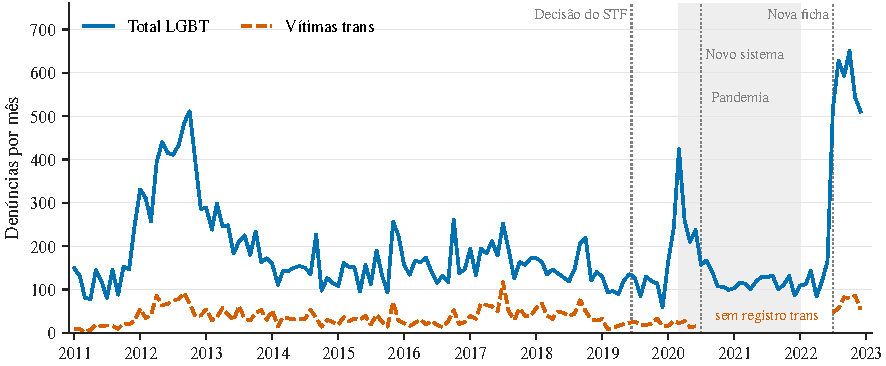
\includegraphics[width=\textwidth]{figuras/fig1_serie_mensal.pdf}
\caption{Denúncias mensais de violência contra pessoas LGBT (linha contínua azul) e contra vítimas trans (linha tracejada vermelha), 2011--2022. As linhas verticais pontilhadas marcam a decisão do STF e as mudanças no sistema de registro; a faixa cinza, a pandemia. Fonte: Disque 100 (ONDH/MDHC).}
\label{fig:serie}
\end{figure}

\subsection{Municípios com números alarmantes}

As denúncias se concentram: as 50 cidades com mais registros somam metade do total. Mas muitas denúncias não significam alto risco: São Paulo tem o maior número absoluto e fica apenas 31\% acima do esperado para o seu porte. Descontados o tamanho da população e o acaso, \textbf{141 municípios tiveram números alarmantes em 2020--2022}, 83 deles com menos de 100 mil habitantes. Os extremos foram Ubaporanga (MG, quase 30 vezes o esperado), Itaporanga (PB, 25), Cabo Frio (RJ, 17), Barbacena (MG, 10) e Campos dos Goytacazes (RJ, 8). Esses municípios formam \textbf{61 aglomerados de alto risco} na Zona da Mata e no Sul de Minas Gerais, na região metropolitana do Rio de Janeiro, no interior de São Paulo, em Goiás e no entorno de João Pessoa (Figura~\ref{fig:mapa}). Entre as 136 cidades com pelo menos 30 registros, 18 cresceram mais rápido que o total nacional, como Juazeiro (BA), Itaporanga (PB) e Barbacena (MG).

\begin{figure}[!htb]
\centering
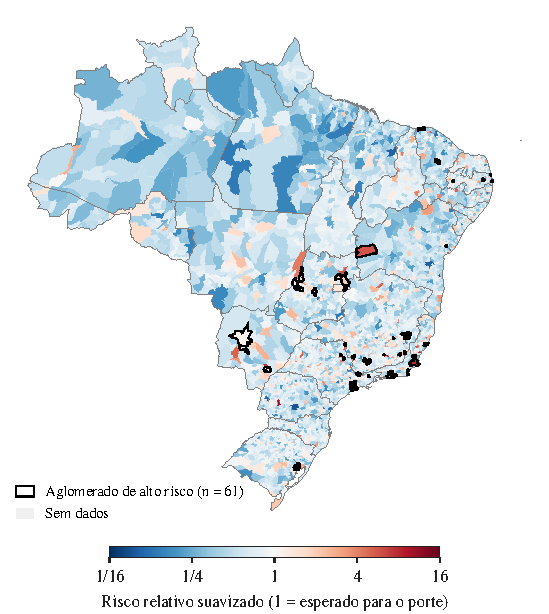
\includegraphics[width=0.62\textwidth]{figuras/fig3_mapa_risco.pdf}
\caption{Risco relativo suavizado de denúncias por município, 2020--2022. Vermelho: mais denúncias do que o esperado para o porte; azul: menos; branco: o esperado. O contorno preto marca os aglomerados de alto risco (Getis-Ord, $p<0{,}05$). Fonte: Disque 100 e IBGE.}
\label{fig:mapa}
\end{figure}

\subsection{Previsão de ondas e fatores associados}

\textbf{É possível prever.} Os três modelos previram melhor do que distribuir as denúncias só pela população, e as regras simples foram piores (Tabela~\ref{tab:validacao}). O LightGBM teve o melhor resultado, com erro 16,7\% menor que a referência, seguido pelo modelo endêmico-epidêmico (14,6\%). Repetir o ano anterior foi a pior estratégia: o número de denúncias de uma cidade varia muito de um ano para o outro, e o passado só ajuda combinado com as características do município. O ganho mais importante está nas ondas: das 20 cidades que o LightGBM apontou a cada ano como mais prováveis de ter uma onda, 37\% de fato a tiveram, contra 15\% usando só a população.

\begin{table}[!htb]
\centering
\caption{Desempenho dos modelos na previsão um ano à frente (média de 2016 a 2022)}
\label{tab:validacao}
{\renewcommand{\arraystretch}{1.2}\small
\begin{tabular}{p{4.6cm} p{2.6cm} p{2.6cm} p{3.0cm}}
\hline
\textbf{Modelo} & \textbf{Redução do erro em relação à população} & \textbf{Acerto das 50 maiores cidades} & \textbf{Acerto entre as 20 cidades apontadas para onda} \\
\hline
LightGBM & 16,7\% & 66\% & 37\% \\
Endêmico-epidêmico & 14,6\% & 63\% & 31\% \\
Extra Trees & 11,3\% & 63\% & 31\% \\
Só população (referência) & -- & 63\% & 15\% \\
Fatia histórica da cidade & $-$14,7\% & 61\% & 29\% \\
Repetir o ano anterior & $-$35,8\% & 55\% & 26\% \\
\hline
\end{tabular}}
\end{table}

\textbf{O que está associado a mais denúncias.} O fator mais forte foi a proporção de domicílios com casais do mesmo sexo, a melhor medida disponível da população LGBT visível: municípios um pouco acima da média nesse indicador têm 13\% mais denúncias (Tabela~\ref{tab:coef}). A densidade teve efeito parecido, e a ouvidoria municipal de direitos humanos se associou a 23\% mais denúncias, sugerindo que um canal institucional facilita a denúncia. Municípios com mais pretos e pardos denunciaram 8\% menos, e Norte e Sul denunciaram menos que o Sudeste. Renda, PIB, desigualdade, homicídios, índice de política LGBT e Processo Transexualizador não mostraram relação com o volume de denúncias.

\begin{table}[!htb]
\centering
\caption{Características associadas a mais (RR $>$ 1) ou menos (RR $<$ 1) denúncias do que o esperado para o porte do município}
\label{tab:coef}
{\renewcommand{\arraystretch}{1.15}\small
\begin{tabular}{p{6.8cm} c c c}
\hline
\textbf{Característica} & \textbf{RR} & \textbf{IC 95\%} & \textbf{Há efeito?} \\
\hline
Casais do mesmo sexo (por desvio-padrão) & 1,13 & 1,08--1,18 & sim \\
Densidade demográfica (por desvio-padrão) & 1,12 & 1,07--1,18 & sim \\
População (por desvio-padrão) & 1,08 & 1,02--1,15 & sim \\
Pretos e pardos (por desvio-padrão) & 0,92 & 0,86--0,98 & sim \\
Tem ouvidoria de direitos humanos & 1,23 & 1,10--1,37 & sim \\
Região Centro-Oeste (em relação ao Sudeste) & 1,36 & 1,17--1,57 & sim \\
Região Sul & 0,72 & 0,64--0,81 & sim \\
Região Norte & 0,58 & 0,48--0,70 & sim \\
Renda domiciliar por pessoa & 1,01 & 0,92--1,10 & não \\
Taxa de homicídios no ano anterior & 0,99 & 0,94--1,03 & não \\
Índice de política LGBT (MUNIC) & 0,99 & 0,96--1,01 & não \\
Processo Transexualizador ativo & 0,71 & 0,34--1,46 & não \\
\hline
\multicolumn{4}{p{12cm}}{\footnotesize Modelo endêmico-epidêmico, 2012--2022. Também incluídos, sem efeito: PIB por pessoa, Gini, população de 15 a 29 anos, estrutura municipal de direitos humanos, capital e Nordeste.}
\end{tabular}}
\end{table}

\textbf{As ondas são locais.} Das denúncias esperadas pelo modelo endêmico-epidêmico, 74\% vêm das características do próprio município, 26\% da inércia do seu histórico e apenas 0,3\% das cidades vizinhas: as ondas nascem e permanecem locais. A cada ano, entre 22 e 52 municípios entraram em alerta, e uma cidade em alerta tem quase 6 vezes mais chance de voltar a ficar em alerta no ano seguinte. Supondo para 2023 o mesmo volume nacional de 2022, a maior chance de onda foi estimada para Barbacena (MG, 40\%).

\subsection{Por que confiar na previsão}

O LightGBM constrói árvores de decisão uma a uma, cada nova árvore corrigindo os erros das anteriores. Nas curvas de aprendizado (Figura~\ref{fig:curvas}), o erro no treino cai continuamente, mas o erro no ano reservado para conferência cai até um ponto mínimo e depois volta a subir (até 11\% acima do mínimo): o treino é interrompido nesse ponto, o que impede que o modelo memorize o passado.

\begin{figure}[!htb]
\centering
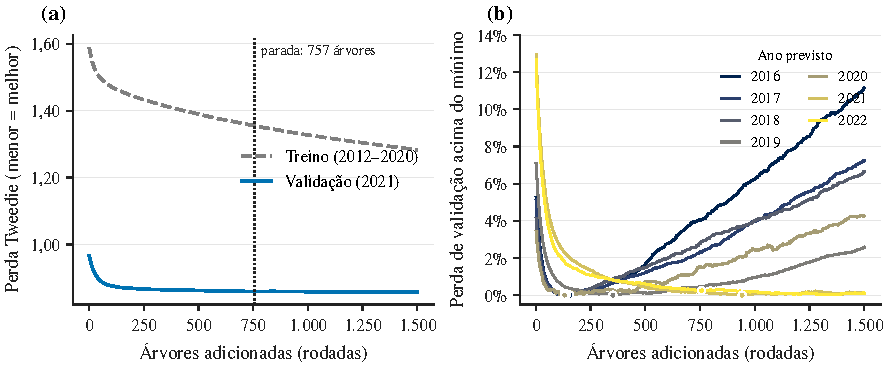
\includegraphics[width=\textwidth]{figuras/fig5_curvas_aprendizado.pdf}
\caption{Aprendizado do LightGBM ao longo das árvores. (a) Previsão de 2022: erro no treino (cinza tracejado) e no ano reservado para conferência (azul); a linha pontilhada marca onde o treino parou. (b) Erro de conferência acima do seu mínimo, para cada ano previsto; os círculos marcam o ponto de parada. Fonte: Disque 100 e IBGE.}
\label{fig:curvas}
\end{figure}

Reamostrando os municípios 2.000 vezes, a redução do erro ficou entre 13,3\% e 20,3\% (IC 95\%). O modelo foi melhor que a referência populacional em todos os sete anos testados e melhor que o endêmico-epidêmico em seis, e o ganho ficou entre 15,7\% e 17,3\% com diferentes parâmetros. Treinado só com as características dos municípios ou só com o histórico, ele já reduz o erro em cerca de 14\%; os vizinhos acrescentam apenas 0,15 ponto, o que confirma que as ondas não se propagam. As previsões são calibradas (o modelo previu 96\% das denúncias que ocorreram) e úteis para priorizar: monitorando só 1\% dos municípios por ano, os escolhidos pelo LightGBM concentram 31\% das ondas, contra 22\% pela população (Figura~\ref{fig:calib}). Por fim, os valores SHAP mostram que o modelo, sem nenhuma hipótese prévia, aprendeu as mesmas relações da Tabela~\ref{tab:coef}: histórico acima do esperado, mais casais do mesmo sexo e maior densidade elevam a previsão. A ablação e o SHAP estão detalhados no relatório técnico que acompanha os códigos.

\begin{figure}[!htb]
\centering
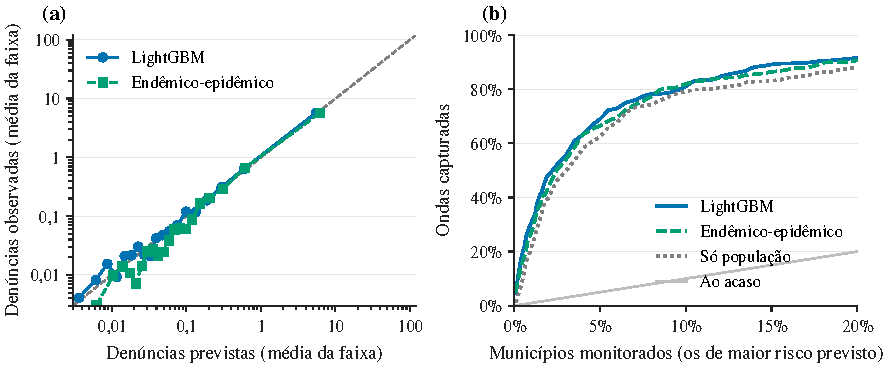
\includegraphics[width=\textwidth]{figuras/fig8_calibracao_captura.pdf}
\caption{(a) Calibração: denúncias previstas e observadas, por faixa de previsão (escala log); a linha tracejada indica previsão perfeita. (b) Percentual das 332 ondas de 2016 a 2022 capturado quando se monitoram os municípios de maior risco previsto; a linha cinza indica a escolha ao acaso. Previsões fora da amostra. Fonte: Disque 100 e IBGE.}
\label{fig:calib}
\end{figure}

\subsection{Violência contra pessoas trans e a decisão do STF}

\textbf{Proporção.} Nos períodos em que a identidade de gênero podia ser registrada, 18\% das denúncias LGBT tinham vítima trans (4.406 de 24.151). Comparando municípios no mesmo ano, essa proporção foi maior no Nordeste (chance 54\% maior que no Sudeste) e menor em cidades mais densas e com mais pretos e pardos. Os municípios alarmantes não diferem dos demais (17\% contra 19\%): as ondas atingem a comunidade LGBT como um todo.

\textbf{Perfil.} A violência contra pessoas trans é mais grave e mais pública (Figura~\ref{fig:perfil}). Em violações contra a vida, a chance de a vítima ser trans é 3 vezes maior, e também é maior na violência sexual (1,7) e física (1,4), na rua, e quando o agressor é desconhecido (1,7) ou profissional e agente de instituição (2,3). Esses registros são também mais incompletos: a raça/cor falta em 30\% deles, contra 16\% nos demais. O modelo distingue os dois grupos de forma moderada (AUC de 0,71), e o LightGBM não foi melhor que a regressão logística.

\begin{figure}[!htb]
\centering
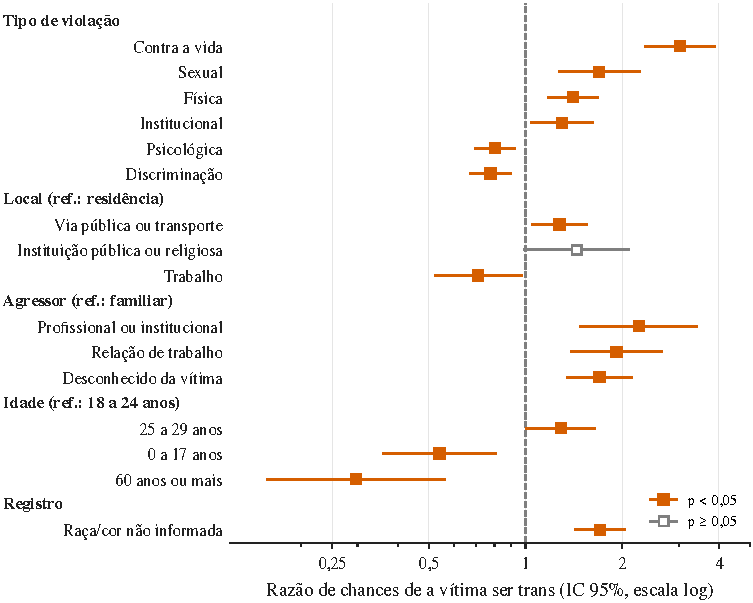
\includegraphics[width=0.85\textwidth]{figuras/fig4_perfil_trans.pdf}
\caption{Quanto cada característica da denúncia aumenta (à direita de 1) ou reduz (à esquerda de 1) a chance de a vítima ser trans. Quadrados cheios: efeito estatisticamente significativo ($p<0{,}05$); quadrados vazados em cinza: sem efeito. As linhas horizontais mostram o intervalo de confiança de 95\%. Fonte: Disque 100 (ONDH/MDHC).}
\label{fig:perfil}
\end{figure}

\textbf{Decisão do STF.} O STF incluiu a transfobia na Lei do Racismo em 13 de junho de 2019. O total de denúncias LGBT não mudou depois da decisão (RR 0,98; IC 95\%: 0,67--1,43). As denúncias com vítima trans caíram 48\%, mas o teste de placebo mostrou que a queda começou em fevereiro de 2019, quatro meses antes, junto com uma mudança no registro da categoria ``travesti''. Com só 13 meses de registros trans após a decisão, não é possível medir o seu efeito. As mudanças administrativas, por outro lado, pesaram muito: a troca de sistema reduziu o volume em 59\%, e o novo formulário o multiplicou por 4,5.


\section{Conclusão}

É possível localizar os municípios em que a violência contra pessoas LGBT é denunciada muito acima do esperado e antecipar onde tendem a surgir ondas. Os 141 municípios alarmantes não são só grandes centros e se agrupam em regiões; o LightGBM foi o melhor modelo e, monitorando 1\% dos municípios, reúne quase um terço das ondas. Denuncia-se mais onde a população LGBT é mais visível, em cidades densas e onde há ouvidoria, e menos no Norte, no Sul e onde há mais pessoas pretas e pardas, o que é compatível com subnotificação, sem que os dados permitam separar menos violência de menos denúncia. As ondas são locais e persistentes. As vítimas trans são 18\% das denúncias, mas sofrem violência mais grave e pública, inclusive por agentes de instituições, e seus registros são os mais incompletos. Não foi possível medir efeito da decisão do STF: mudanças no registro pesaram mais que o marco legal. Como trabalhos futuros, propomos manter um campo estável de identidade de gênero no Disque 100, cruzar as denúncias com o Sinan e o SIM e testar a previsão com os dados de 2023 em diante.


\appendix

\section{Fórmulas}

{\small
Índices: $i$ município, $t$ ano, $m$ mês, $k$ denúncia. $y_{it}$: denúncias LGBT observadas; $N_t$: total nacional no ano; $P_{it}$: população. Variáveis contínuas padronizadas (média 0, desvio-padrão 1); $e^{\beta}$ é a razão de taxas ou de chances.

\textbf{A1. Valor esperado.} $E_{it} = N_t\, P_{it} / \sum_j P_{jt}$.

\textbf{A2. Risco relativo suavizado} \cite{marshall:1991}. $\widehat{RR}_i = (y_i+\alpha)/(E_i+\beta)$ e $P(RR_i>1) = 1 - F_{\text{Gama}}(1;\, y_i+\alpha,\, E_i+\beta)$, com $\alpha$ e $\beta$ estimados pelo método dos momentos. Alarmante: $P(RR_i>1) > 0{,}95$.

\textbf{A3. Getis-Ord} \cite{getis_ord:1992}.
\begin{equation*}
G_i^{*} = \frac{\sum_{j} w_{ij}\, \widehat{RR}_j - \bar{R}\sum_j w_{ij}}{s\sqrt{\left[n\sum_j w_{ij}^2 - \left(\sum_j w_{ij}\right)^2\right]/(n-1)}}
\end{equation*}
com $w_{ij}=1$ para o próprio município e seus 10 vizinhos mais próximos ($\mathcal{V}(i)$) e 0 nos demais; $\bar{R}$ e $s$: média e desvio-padrão do risco relativo. Significância por 999 permutações; aglomerado alto se $G_i^{*}>0$, $p<0{,}05$ e $\widehat{RR}_i>1$.

\textbf{A4. Modelo endêmico-epidêmico Binomial Negativo} \cite{held_hohle_hofmann:2005}.
\begin{equation*}
y_{it} \sim \text{BN}(\mu_{it}, \theta), \quad
\mu_{it} = \underbrace{e^{\mathbf{x}_{it}^{\top}\boldsymbol{\beta}} E_{it}}_{\text{estrutural}}
+ \underbrace{\lambda_i\, r_t\, y_{i,t-1}}_{\text{inércia}}
+ \underbrace{\phi_i\, r_t\, \bar{y}_{\mathcal{V}(i),t-1}}_{\text{vizinhança}}, \quad r_t = \frac{N_t}{N_{t-1}}
\end{equation*}
em que $\mathbf{x}_{it}$ são as características do município (Tabela~\ref{tab:fontes}), $\log\lambda_i$ e $\log\phi_i$ dependem do log da população e $\theta$ é a dispersão; estimação por máxima verossimilhança. O LightGBM usa perda Tweedie (potência 1,3) com $\log E_{it}$ como termo fixo. Métrica: desvio de Poisson $D = \frac{2}{n}\sum \left[y \log(y/\hat{\mu}) - (y-\hat{\mu})\right]$; redução do erro $= 1 - D_{\text{modelo}}/D_{\text{só população}}$.

\textbf{A5. Onda e alerta.} Onda: $y_{it} \ge 5$ e $y_{it} \ge 2E_{it}$. Alerta \cite{farrington:1996}: $y_{it} > q_{0,95}(\hat{\mu}_{it}, \hat{\theta})$ e $y_{it}\ge 3$, em que $q_{0,95}$ é o percentil 95 da Binomial Negativa prevista por A4.

\textbf{A6. Proporção de vítimas trans.} $y^{\text{trans}}_{it} \sim \text{Binomial}(n_{it}, \pi_{it})$, $\text{logit}(\pi_{it}) = \gamma_t + \mathbf{x}_{it}^{\top}\boldsymbol{\beta}$, com $n_{it}$ as denúncias LGBT em períodos com registro de identidade trans e $\gamma_t$ o efeito do ano; quase-binomial, erros-padrão agrupados por município.

\textbf{A7. Perfil da vítima.} $\text{logit}\, P(\text{trans}_k = 1) = \gamma_{t(k)} + \mathbf{v}_k^{\top}\boldsymbol{\beta}$, com $\mathbf{v}_k$ o tipo de violação, local, relação com o agressor, idade, raça/cor e região da denúncia.

\textbf{A8. Série temporal interrompida} \cite{bernal:2017}.
\begin{equation*}
\log \mathrm{E}[Y_m] = \beta_0 + \beta_1 m + \beta_2 D_m + \beta_3 (m-m_0) D_m + \boldsymbol{\gamma}^{\top}\mathbf{c}_m + \textstyle\sum_{k=1}^{2}\left[\delta_k \sin\frac{2\pi k\,\text{mês}}{12} + \eta_k \cos\frac{2\pi k\,\text{mês}}{12}\right]
\end{equation*}
com $D_m = 1$ a partir de junho de 2019 ($m_0$); $\mathbf{c}_m$: pandemia, novo sistema (jul/2020) e nova ficha (jul/2022). Erros de Newey-West (6 defasagens). No placebo, $m_0$ percorre os meses de 2018 e 2019.
}


\bibliographystyle{sbc}
\bibliography{sbc-template,referencias_metodo}

\end{document}
